CPU-Rechenzeit ist eine wertvolle Ressource und muss finanziert werden. Weiterhin erfreut es den (ungeduldigen) Anwender, wenn das Ergebnis einer quantenchemischen Rechnung möglichst schnell erhalten wird. Aus diesem Grund ist die Effizienzsteigerung immer ein aktuelles Forschungsgebiet. Eine Möglichkeit, Berechnungen effizienter durchzuführen, ist durch das Einführen von Näherungen gegeben. Diese Vereinfachen die zu berechnenden Größen und führen damit schneller zu Resultaten. Eine weit gebräuchliche Näherung ist mit der \ac{ri}-Näherung gegeben\supercite{vahtras1993integral}, welche im Ursprung auf Dunlap\supercite{dunlap1979some} und Whitten\supercite{whitten1973coulombic} zurückzuführen ist. Die Übertragung dieser Methode auf die Berechnung von chemischen Abschirmungskonstanten, sowie eine weitere Beschleunigung der Näherung durch eine Multipolentwicklung, sind in den folgenden Kapiteln \ref{ri} und \ref{marij} erläutert. Jedoch darf die Genauigkeit des Resultats nicht unter diesen Näherungsmethoden leiden. Aus diesem Grund wurde die Effizienz und die erhaltene Genauigkeit in Kapitel \ref{genauigkeit} untersucht. Optimierungen des Programmcodes, effizientes Abschätzen verschwindender Integralbeiträge und Parallelisierung des Programmcodes stellen weitere Möglichkeiten dar, um die Effizienz zu verbessern und sind in Kapitel \ref{paraopt} zusammengefasst. 

\bigskip
Unabhängig von der Verbesserung der Effizienz kann für die Implementierung von Integralen, welche nach den Komponenten des Magnetfeldes abgeleitet werden müssen, folgendes ausgenutzt werden. Als Beispiel sollen die abgeleiteten Kern-Elektron-Wechselwirkungsintegrale betrachtet werden. Mit der Beziehung $\vec{r}=\vec{r_\mu}+\vec{R}_\mu$ gilt für sie

\begin{equation}\label{eq:vmunudb}
\begin{aligned}
&\frac{\partial}{\partial B_\beta}\left(\left\langle\chi_{\mu}\left\vert\hat{V}_{\textrm{Ke}}\right\vert\chi_{\nu}\right\rangle\right)_{\vec{B}=0}=\frac{\iu}{2c}\left\langle\chi_{\mu}\left\vert\left(\vec{R}_{\mu\nu}\times\vec{r}\right)\hat{V}_{\textrm{Ke}}\right\vert\chi_{\nu}\right\rangle\\
&=\frac{\iu}{2c}\left\langle\chi_\mu^{\vec{B}=0}\left\vert\left(\vec{R}_{\mu\nu}\times\vec{r}_\mu\right)_\beta\hat{V}_{\textrm{Ke}}\right\vert\chi_\nu^{\vec{B}=0}\right\rangle+\frac{\iu}{2c}\left(\vec{R}_\mu\times\vec{R}_\nu\right)_\beta\left\langle\chi_{\mu}^{\vec{B}=0}\left\vert\hat{V}_{\textrm{Ke}}\right\vert\chi_{\nu}^{\vec{B}=0}\right\rangle.
\end{aligned}
\end{equation}

Bei der Verwendung von gewöhnlichen, atomzentrierten Basisfunktionen der Form

\begin{equation}
\chi_\mu^{\vec{B}=0}=x_\mu^l y_\mu^m z_\mu^n e^{-\zeta\vec{r}_\mu^2},
\end{equation}

wobei $\zeta$ der Exponent der Basisfunktion ist, können die Abgeleiteten Integrale aus den nicht abgeleiteten Integralen durch Multiplikation mit dem Faktor $\frac{\iu}{2c}\left(\vec{R}_\mu\times\vec{R}_\nu\right)$ (zweiter Term auf der rechten Seite in Gleichung (\ref{eq:vmunudb})) und aus den nicht abgeleiteten Integralen, bei denen entsprechend die l-Quantenzahl ($l$, $m$, $n$) um 1 erhöht wurde (zweiter Term auf der rechten Seite in Gleichung (\ref{eq:vmunudb})), berechnet werden. Letztere werden auch in ähnlicher Form (mit anderem Vorfaktor) bei der Berechnung des kartesischen Gradienten erhalten, sodass für ihre Berechnung vorhandene Gradientenroutinen modifiziert werden können. Alternativ lassen sie sich jedoch auch durch Modifikation der Routinen für die Berechnung der Energie erhalten. 

\section{Die RI-Methode für chemische Abschirmungskonstanten}\label{ri}
Die \ac{ri}-Näherung stellt in der \ac{scf}-Prozedur ein bewährtes Näherungsverfahren zur Berechnung der Zweielektronenintegrale dar. Diese setzen sich aus dem Coulombterm und dem Austauschterm zusammen und deren Berechnung ist der zeitaufwändigste Schritt während des Verfahrens. Insbesondere der Coulombterm lässt sich durch das Anwenden der \ac{ri}-Näherung deutlich effizienter berechnen. Dies gilt bereits für Basissätze von \textit{double}-$\zeta$ Qualität und wird für größere Basissätze noch effizienter. Prinzipiell kann die Näherung auch für den Austauschterm angewendet werden, die Rechenzeiten verkürzen sich jedoch erst deutlich bei größeren Basissätzen ab \textit{quadruple}-$\zeta$ Qualität. Wird nur der Coulombterm oder nur der Austauschbeitrag angenähert, so wird von \ac{ri}-J oder \ac{ri}-K gesprochen, bzw. \ac{ri}-JK wenn die Näherung für beide Terme angewendet wird. 

Auch bei der Berechnung chemischer Abschirmungskonstanten ist die Berechnung der abgeleiteten Zweielektronenintegrale zeitbestimmend. Dies gilt insbesondere dann, wenn reine \ac{dft}-Funktionale (d.h. keine Hybrid-Funktionale mit Hartree-Fock-Austausch) verwendet werden, da für sie im Rahmen der \textit{uncoupled}-\ac{dft} keine \ac{cphf}-Gleichungen gelöst werden müssen. Die \ac{ri}-Näherung lässt sich auch auf die abgeleiteten Zweielektronenintegrale übertragen, wobei die Näherung in dieser Arbeit lediglich auf den abgeleiteten Coulombterm übertragen wird. Das getrennte Berechnen der Coulomb- und Austauschterme hat weiterhin den Vorteil, dass für die konventionelle Berechnung des Austauschs eine effizientere Integralabschätzung angewendet werden kann. Dies ist durch den schnelleren Abfall des Austauschs im Vergleich zur Coulombwechselwirkung begründet. Folglich kann damit durch Anwenden der \ac{ri}-J-Näherung auch der Austausch effizienter Berechnet werden. Weiteres dazu wird in Kapitel \ref{paraopt} erläutert. 
	\subsection{Theorie}
	An dieser Stelle sollen zunächst die grundlegende Idee der Näherung und die daraus resultierenden Formeln aus \supercite{vahtras1993integral} wiedergegeben werden. Im Anschluss daran folgt die Übertragung auf die nach den Komponenten des Magnetfeldes abgeleiteten Coulombintegrale. 
	
	Die Berechnung der Coulombintegrale skalieren formell mit der Anzahl der Baisfunktionen $N_\textrm{BF}$ wie $\mathcal{O}(N_\textrm{BF}^4)$. Durch Anwenden der \ac{ri}-Näherung lässt sich das formelle Skalierungsverhalten um eine Potenz erniedrigen. Die Vierzentrenintegrale lassen sich als Summe des Produkts von Zwei- und Dreizentrenintegralen schreiben, welche wie $\mathcal{O}(N_\textrm{BF}^2)$ und $\mathcal{O}(N_\textrm{BF}^3)$ skalieren. Um diese zu erreichen, wird das Produkt zweiter Basisfunktionen $\chi_\mu$ und $\chi_\nu$ durch die Linearkombination von sogenannten atomzentrierten Auxiliarbasisfunktionen $P$ angenähert
	
	\begin{equation}
	\gamma_{\mu\nu}=\chi_\mu\chi_\nu\approx\sum_PC^P_{\mu\nu}P=\tilde{\gamma}_{\mu\nu}.
	\end{equation}
	
	Durch die Minimierung des Fehlers
	\begin{equation}
	\delta\gamma_{\mu}\nu = \gamma_{\mu\nu}-\tilde{\gamma}_{\mu\nu}
	\end{equation}
	
	wird letztendlich ein genäherter Ausdruck für die Vierzentrenintegrale erhalten
	
	\begin{equation}\label{eq:munukalari}
	\left(\chi_\mu\chi_\nu\vert\chi_\kappa\chi_\lambda\right)\approx\sum_{PQ}^{N_{\textrm{AuxBF}}}\left(\chi_\mu\chi_\nu\vert P\right)\left(P\vert Q\right)^{-1}\left(Q\vert\chi_\kappa\chi_\lambda\right).		
	\end{equation}
	Für eine effiziente Berechnung der Matrixelemente der Coulombmatrix $J_{\mu\nu}$, wofür Gleichung (\ref{eq:munukalari}) noch mit der Dichtematrix $D_{\kappa\lambda}$ gespurt werden muss, wird zunächst die inverse $\left(P\vert Q\right)^{-1}$-Matrix gebildet und mit den Dreizentrenintegralen $\left(Q\vert\chi_\kappa\chi_\lambda\right)$ sowie der Dichtematrix zur intermediären Größe $\Gamma_P$ verarbeitet
	\begin{equation}
	\Gamma_P=\sum_Q^{N_{\textrm{AuxBF}}}\left(P\vert Q\right)^{-1}\sum_{\kappa\lambda}D_{\kappa\lambda}\left(Q\vert\chi_\kappa\chi_\lambda\right).
	\end{equation}
	Die eigentliche Berechnung von $J_{\mu\nu}$ erfolgt durch Spuren der Dreizentrenintegrale $\left(\chi_\mu\chi_\nu\vert P\right)$ mit $\Gamma_P$
	\begin{equation}
	J_{\mu\nu}=\sum_{\kappa\lambda}D_{\kappa\lambda}\left(\chi_\mu\chi_\nu\vert\chi_\kappa\chi_\lambda\right)\approx\sum_{P}^{N_{\textrm{AuxBF}}}\left(\chi_\mu\chi_\nu\vert P\right)\Gamma_P=J_{\mu\nu}^{\textrm{RI}}.
	\end{equation}
	Im Vergleich zu den Fehlern der Methoden sind die Fehler, die durch diese Näherung gemacht werden, klein und von wenig Bedeutung.\supercite{eichkorn1995auxiliary} Die \ac{ri}-Näherung lässt sich nun auch auf den nach den Komponenten des Magnetfeldes abgeleiteten Coulombterm übertragen. Wie bereits zuvor erwähnt, gilt
	
	\begin{equation}\label{eq:jmunudb}
	\begin{aligned}
	J_{\mu\nu}^{B_\beta}=&\frac{\partial}{\partial B_\beta}\left(\sum_{\kappa\lambda}D_{\kappa\lambda}\left(\chi_\mu\chi_\nu\vert\chi_\kappa\chi_\lambda\right)\right)_{\vec{B}=0}\\
	=&\sum_{\kappa\lambda}\left[D_{\kappa\lambda}^{B_\beta}\left(\chi_\mu^{\vec{B}=0}\chi_\nu^{\vec{B}=0}\vert\chi_\kappa^{\vec{B}=0}\chi_\lambda^{\vec{B}=0}\right)+D_{\kappa\lambda}\left(\overline{\chi_\mu\chi_\nu}\vert\chi_\kappa^{\vec{B}=0}\chi_\lambda^{\vec{B}=0}\right)_{\beta}\right.\\
    &+\left.D_{\kappa\lambda}\left(\chi_\mu^{\vec{B}=0}\chi_\nu^{\vec{B}=0}\vert\overline{\chi_\kappa\chi_\lambda}\right)_{\beta}\right]\\
    =&\sum_{\kappa\lambda}D_{\kappa\lambda}\left(\overline{\chi_\mu\chi_\nu}\vert\chi_\kappa^{\vec{B}=0}\chi_\lambda^{\vec{B}=0}\right)_{\beta}
	\end{aligned}
	\end{equation}
	da bei den Verschwindenden Termen in Gleichung (\ref{eq:jmunudb}) jeweils die Spur des Produkts einer symmetrischen mit einer antisymmetrischen Matrix sind. Es muss folglich nur die linke Seite des Integrals, also nur die Basisfunktionen $\chi_\mu$ und $\chi_\nu$, abgeleitet werden. Das Einsetzen der \ac{ri}-Näherung liefert daher
	
	\begin{equation}\label{eq:jmunudbri}
	\begin{aligned}
	J_{\mu\nu}^{B_\beta}\approx &\sum_{PQ}^{N_{\textrm{AuxBF}}}\left(\overline{\chi_\mu\chi_\nu}\vert P\right)_\beta\left(P\vert Q\right)^{-1}\sum_{\kappa\lambda}D_{\kappa\lambda}\left(Q\left\vert\chi_\kappa^{\vec{B}=0}\chi_\lambda^{\vec{B}=0}\right.\right)\\
	=&\sum_{P}^{N_{\textrm{AuxBF}}}\left(\overline{\chi_\mu\chi_\nu}\vert P\right)_\beta\Gamma_P=J_{\mu\nu}^{B\beta ,\textrm{RI}}.
	\end{aligned}
	\end{equation}
	\vfill
	\subsection{Implementierung}
	Die intermediäre Größe $\Gamma_P$, welche für die abgeleiteten Coulombintegrale in Gleichung (\ref{eq:jmunudbri}) benötigt wird, kann auf die ganz konventionelle Art berechnet werden, wie es beispielsweise auf für die Berechnung der Energie während des \ac{scf}-Verfahrens notwendig ist. Neben den Trivialitäten, wie dem Modifizieren des Moduls zum Einlesen der Auxiliarbasissatzinformationen, müssen zusätzlich noch die abgeleiteten Dreizentrenintegrale $\left(\overline{\chi_\mu\chi_\nu}\vert P\right)$ implementiert werden. Diese sind von der Form
	
	\begin{equation}\label{eq:3centintdb}
	\begin{aligned}
	\left(\left.\overline{\chi_\mu\chi_\nu}\right\vert P\right)_\beta=&\frac{\iu}{2c}\left(\left.\left(\vec{R}_{\mu\nu}\times\vec{r}\right)_\beta\chi_\mu^{\vec{B}=0}\chi_\nu^{\vec{B}=0}\right\vert P\right)\\
	=&\frac{\iu}{2c}\left(\left.\left(\vec{R}_{\mu\nu}\times\vec{r}_\mu\right)_\beta\chi_\mu^{\vec{B}=0}\chi_\nu^{\vec{B}=0}\right\vert P\right)\\
	&+\frac{\iu}{2c}\left(\left.\vec{R}_\mu\times\vec{R}_\nu\right)_\beta\left(\chi_\mu^{\vec{B}=0}\chi_\nu^{\vec{B}=0}\right\vert P\right)
	\end{aligned}
	\end{equation}
	und lassen sich damit aus den nicht abgeleiteten Integralen berechnen, wobei beachtet werden muss, dass die $l$-Quantenzahl für $\chi_\mu$ im ersten Term auf der rechten Seite in Gleichung (\ref{eq:3centintdb}) um 1 erhöht werden muss. Integrale dieser Form werden bereits in den Routinen zur Berechnung des kartesischen Gradienten mit \ac{ri}-Näherung benötigt. Diese Routinen wurden entsprechend modifiziert um alle nach den Komponenten des Magnetfeldes abgeleiteten Integrale zu erhalten. In der Abbildung \ref{abb:programmstrukur_ri} ist eine schematische Darstellung der wichtigsten übertragenen, modifizierten und neuen Routinen in das \texttt{mpshift} Modul gegeben. Alte Routinen sind in blau, neue Routinen in grün, modifizierte Routinen in orange und unverändert aus anderen Modulen übertragene Routinen in rot dargestellt. Die Funktion der einzelnen Routinen sei im Folgenden erläutert.
	
	\begin{itemize}[leftmargin=65pt]
	    \item[\texttt{riprep}:] Routine zur Vorbereitung der notwendigen Größen und Felder für die Berechnung von $J_{\mu\nu}^{B\beta ,\textrm{RI}}$ mit der \ac{ri}-Näherung. 
	    \item[\texttt{lp2sym}:] Berechnung der $\left(P\vert Q\right)$-Matrix.
	    \item[\texttt{sichol}:] Cholesky-Zerlegung der $\left(P\vert Q\right)$-Matrix, da für die spätere Verarbeitung nicht explizit die Inverse $\left(P\vert Q\right)^{-1}$-Matrix berechnet wird.
	    \item[\texttt{twoder}:] Treiberroutine zur Berechnung von $J_{\mu\nu}^{B\beta ,\textrm{RI}}$. Es wird zunächst die intermediäre Größe $\Gamma_P$ aus der Cholesky-Zerlegung von $\left(P\vert Q\right)$ und aus $\Gamma_Q$ (siehe \texttt{lpdrc1}) berechnet und im Anschluss folgt die eigentliche Berechnung von $J_{\mu\nu}^{B\beta ,\textrm{RI}}$.
	    \item[\texttt{lpdrc1}:] Berechnung der Dreizentrenintegrale. Diese werden direkt mit der Dichtematrix kontrahiert, sodass die Größe $\Gamma_Q=\sum_{\kappa\lambda}D_{\kappa\lambda}\left(Q\vert\chi_\kappa\chi_\lambda\right)$ erhalten wird.
	    \item[\texttt{cslp3\_omp}:] Übergeordnete Routine zur Unterscheidung zwischen sequentieller und paralleler Ausführung des Moduls.
	    \item[\texttt{cslp3}:] Berechnung der Abgeleiteten Dreizentrenintegrale $\left(\left.\overline{\chi_\mu\chi_\nu}\right\vert P\right)$. Schleife über alle Schalentripel $i,j,k$.
	    \item[\texttt{csasra3}:] Schleife über die primitiven Basisfunktionen $\chi_\mu^{\vec{B}=0}$ und $\chi_\nu^{\vec{B}=0}$ und primitiven Auxiliarbasisfunktionen $P$
	    \item[\texttt{csgasram}:] Berechnung der eigentlichen Dreizentrenintegrale für aktuelles Tripel primitiver Basisfunktionen $\chi_\mu^{\vec{B}=0}$ und $\chi_\nu^{\vec{B}=0}$ und primitiver Auxiliarbasisfunktion $P$ für das aktuelle Schalentripel $i,j,k$.
	    \item[\texttt{crosscs}:] Berechnung des Kreuzprodukts in Gleichung (\ref{eq:3centintdb}) für beliebige Schalenpaare $i,j$. Die Berechnung der Kreuzprodukte für die Schalenkombinationen $s,s$ und $s,p$ erfolgt explizit in \texttt{cspl3}.
	    \item[\texttt{dftfck}:] Addition der Beiträge der Schalenpaare $i,j$ auf die Fockmatrix.
	\end{itemize}
	
\begin{figure}[ht!]
\centering
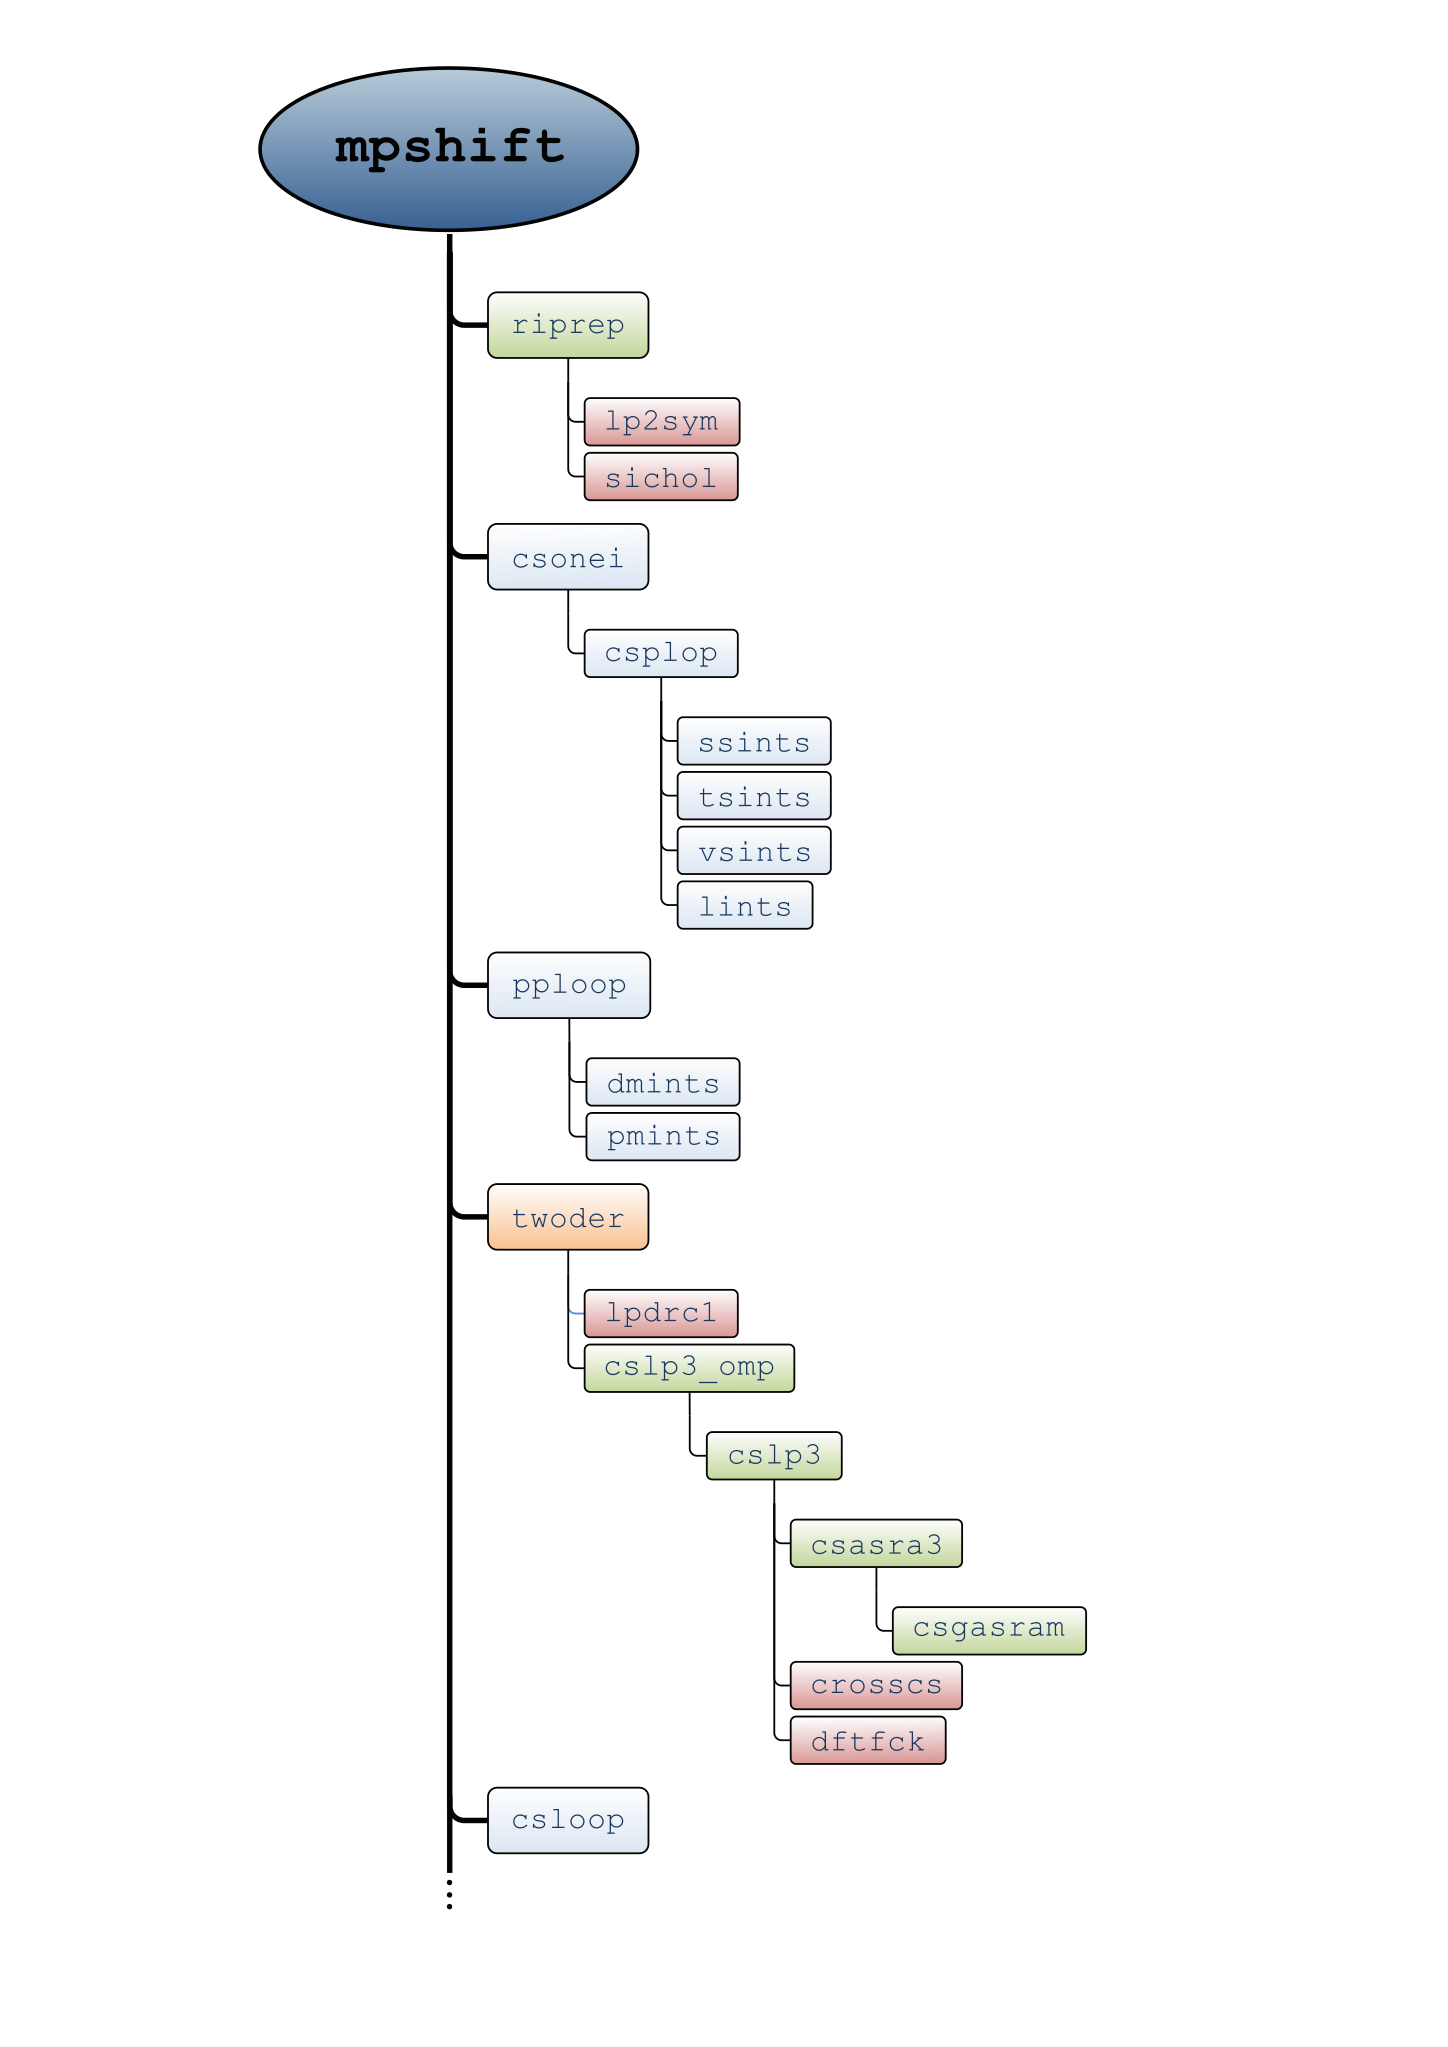
\includegraphics[width=0.6\textwidth]{programmstruktur_ri}
\captionsetup{figurewithin = chapter}
\captionsetup{font=small, labelfont=bf}\caption[RI-J Routinen für chemische Abschirmungskonstanten]{Schematische Darstellung der wichtigsten Routinen für die \ac{ri}-Näherung zur berechnung chemischer Abschirmungskonstanten im Modul \texttt{mpshift}. Alte Routinen sind in blau, neue Routinen in grün, modifizierte Routinen in orange und unverändert übertragene Routinen in rot dargestellt.}
\label{abb:programmstrukur_ri}
\end{figure}

\section{Die MARI-J Methode für chemische Abschirmungskonstanten}\label{marij}
	\subsection{Theorie}
	\subsection{Implementierung}

\section{Seminumerischer Austausch}
	\subsection{Theorie}
	\subsection{Implementierung}
	
\section{Parallelisierung und weitere Optimierungen}\label{paraopt}
Bei bestimmten Verbindungen kann es von Interesse sein, die chemischen Abschirmungskonstanten nur für eine Auswahl an Atomen zu berechnen. Beispielsweise wenn nur eine bestimmte Atomsorte von Interesse ist oder lediglich die chemische Verschiebung in einem bestimmten Bereich untersucht werden soll. In diesen Fällen kann es von Nutzen sein, nur die Beiträge für besagte Atome zu berechnen. Aus diesem Grund wurde das Modul \texttt{mpshift} um die Möglichkeit ergänzt, eine Vorauswahl der zu berechnenden Atome zu treffen. Im Programmcode selbst ist dies auf die einfache Weise realisiert, dass die Ableitungen nach den Komponenten der Kernmomente sowie der gesamte Abschirmungstensor nur für die ausgewählten Atome berechnet wird. Dies kann durch Hinzufügen des Keywords \texttt{\$nucsel} im \texttt{control}-File erreicht werden. Durch die Eingabe von \texttt{\$nucsel "N","Fe"} lassen sich beispielsweise die chemischen Abschirmungskonstanten für alle Sickstoff- und Eisenatome im Molekül berechnen. Mit \texttt{\$nucsel 1,3,5-8} erfolgt die Berechnung für die Atome Nummer 1,3,5-8 im \texttt{coord}-File. Sind in größeren organischen Molekülen, welche von Wasserstoff- und Kohlenstoffatomen dominiert sind, nur die $^1$H bzw. $^13$C Abschirmungskonstanten von Interesse, so bringt dieses vorgehen in der Regel jedoch kaum eine Zeitersparnis und es können direkt alle Atome berechnet werden. Umgekehrt lassen sich auf diese Weise auch Elemente aus der Rechnung herausnehmen, welche ohnehin nicht von Interesse sind, aber gegebenenfalls für ein schlechtes Konvergenzverhalten während der \ac{cphf}-Iterationen sorgen.

\bigskip
Das bisherige, standardmäßige Auswählen des ersten Atoms im \texttt{coord}-File für den Konvergenztest bei den \ac{cphf}-Iterationen lässt sich ebenfalls optimieren. In der Praxis hat sich herausgestellt, dass insbesondere für schwere Elemente mehr Iterationen benötigt werden, bis die Konvergenz erreicht wurde. Dies liegt auch daran, dass die Absolutwerte für die chemischen Abschirmungskonstanten dieser Elemente mit zunehmender Ordnungszahl steigen. Die Konvergenz wurde aber Standardmäßig auf eine Änderung von weniger als \unit[$1\times 10^{-2}$]{ppm} gesetzt, unabhängig von Element. Hierfür wurde ein Faktor eingeführt, welcher die Ordnungszahl des entsprechenden Elements berücksichtigt und die Konvergenz für Elemente mit hoher Ordnungszahl ein wenig lockert. Weiterhin hat sich herausgestellt, dass Atome die weit vom Koordinatenursprung entfernt sind, ebenfalls länger bis zur Konvergenz benötigen. Daher erfolgt die Atomauswahl für den Konvergenztest bei den \ac{cphf}-Iterationen dermaßen, dass zunächst das schwerste Element im Molekül gesucht wird. Sollte es davon mehrere geben, dann wird das Atom ausgewählt, welches am weitesten vom Ursprung entfernt liegt. Dieses Vorgehen hat den Vorteil, dass in der Regel nur in den letzten beiden Iterationen die chemische Verschiebung für alle Atome berechnet werden muss, um zu überprüfen, ob alle Atome bereits konvergiert sind. Da der kritischste Fall zu diesem Zeitpunkt in der Regel bereits zur Konvergenz gebracht werden konnte, ist dies in der Regel gegeben.

\bigskip
Wird die \ac{ri} bzw. \ac{marij}-Methode in einer Hartree-Fock bzw. Hybrid-\ac{dft} Rechnung verwendet, so wird der Austauschbeitrag unabhängig vom Coulombbeitrag berechnet. Für ersteren kann jedoch eine härtere Integralabschätzung angewendet werden, als für den Coulombbeitrag. Aus diesem Grund wurden die Integralabschätzungen aus der Routine \texttt{shloop\_k}, welche ungestörten Austauschmatrixelemente in einer \ac{scf} oder während der \ac{cphf}-Iterationen berechnet, in die Routine \texttt{csloop} übertragen. Auf diese Weise kann die Berechnung kleiner bzw. später verschwindender Matrixelemente vermieden werden. 

\bigskip
Neben einer effizienten Programmierung und dem Einführen von Näherungen wie beispielsweise bei der \ac{ri} bzw. \ac{marij}-Methode, kann die Wartezeit des Nutzers auch durch eine Parallelisierung des Programmcodes reduziert werden. Dies ist insofern von besonderer Bedeutung, dass heutige Computer immer mehr CPUs zur Verfügung haben. Selbst in gewöhnlichen Desktop PCs oder Notebooks finden sich häufig mindestens 4 CPUs. Aus diesem Grund wurden die zeitaufwändigsten Routinen im \texttt{mpshift} Modul mit OpenMP\supercite{dagum1998openmp} in Zusammenarbeit mit Fabian Mack parallelisiert. Im Einzelnen betrifft dies die Routinen \texttt{becke}, \texttt{csloop}, \texttt{cslp3\_omp}, \texttt{csplop},\texttt{shloop\_k} \texttt{p3loop} und \texttt{pploop}. Die Routinen \texttt{csplop}, \texttt{p3loop} und \texttt{pploop} besitzen üblicherweise folgende grundlegende Schleifenstruktur.\\
\\
\texttt{do i=1,N$_{\texttt{Schal}}$}\\ 
\null\quad\texttt{do j=1,N$_{\texttt{Schal}}$}\\ 
\null\quad\quad\texttt{do $\mu$=1,N$_{\texttt{Prim BF}}$}\\ 
\null\quad\quad\quad\texttt{do $\mu$=1,N$_{\texttt{Prim BF}}$}\\
\null\quad\quad\quad\quad \texttt{Auszuführender Programmcode}\\ 
\null\quad\quad\quad\texttt{end do}\\ 
\null\quad\quad\texttt{end do}\\ 
\null\quad\texttt{end do}\\ 
\texttt{end do}\\
\\
Die äußeren beiden Schleifen laufen dabei über alle Schalen N$_{\texttt{Schal}}$ und die beiden inneren Schleifen laufen über die primitiven Basisfunktionen. Für die Routine \texttt{cslp3\_omp} kommt jeweils eine weitere Schleife für die Auxiliarschale und die primitiven Auxiliarbasisfunktionen hinzu. Bei den Vierzentrenroutinen \texttt{csplop} und \texttt{shloop\_k} sind es jeweils zwei weitere Schleifen für die Schalen und die primitiven Basisfunktionen. Bei der Parallelisierung wurde nun in der Regel so vorgegangen, dass die äußersten Schleifen über die Schalen parallelisiert wurden:\\
\\
\texttt{\$OMP PARALLEL}\\
\texttt{\$OMP DO SCHEDULE (DYNAMIC)}\\
\texttt{do i=1,N$_{\texttt{Schal}}$}\\ 
\null\quad\texttt{do j=1,N$_{\texttt{Schal}}$}\\ 
\null\quad\quad\texttt{do $\mu$=1,N$_{\texttt{Prim BF}}$}\\ 
\null\quad\quad\quad\texttt{do $\mu$=1,N$_{\texttt{Prim BF}}$}\\
\null\quad\quad\quad\quad \texttt{Auszuführender Programmcode}\\ 
\null\quad\quad\quad\texttt{end do}\\ 
\null\quad\quad\texttt{end do}\\ 
\null\quad\texttt{end do}\\ 
\texttt{end do}\\
\texttt{\$OMP END DO}\\
\texttt{\$OMP END PARALLEL}\\
\\


\section{Genauigkeit und Effizienz}\label{genauigkeit}